\documentclass[11pt]{article}
\usepackage[margin=1in]{geometry}
\usepackage{amsmath,amssymb,amsthm,mathtools}
\usepackage{graphicx}
\usepackage{float}
\usepackage{microtype}
\usepackage[hidelinks]{hyperref}

\newtheorem{theorem}{Theorem}
\newtheorem{lemma}[theorem]{Lemma}
\newcommand{\C}{\mathbb C}
\newcommand{\tr}{\operatorname{tr}}
\newcommand{\dEt}{\operatorname{dEt}}

\title{The Weighted-Ellipsoid Determinant Trace Is Exactly $2/3$}
\author{Partial-result packet for arXiv:2012.11115}
\date{12 August 2026}

\begin{document}
\maketitle

\begin{center}
\fbox{\begin{minipage}{0.9\textwidth}
\textbf{Status: candidate substantial partial result, likely valid; human
review requested.}
For every $\lambda\ge4$, the coordinate-multiplication pair on the weighted
Bergman space of the source ellipsoid
$\mathbb B_{2,1}=\{(z_1,z_2):|z_1|^2+|z_2|<1\}$ has determinant-commutator
trace exactly $2/3$.  This converts the source's numerical evidence into a
proof and verifies its spectral-volume conjecture with equality for its only
non-ball model.  The conjecture for arbitrary tuples remains open.
\end{minipage}}
\end{center}

\section{Source conjecture and numerical test case}

The source is G.~Misra, P.~Pramanick, and K.~B.~Sinha,
\emph{A trace inequality for commuting tuple of operators},
arXiv:2012.11115 \cite{MPS}.  For a commuting $d$-tuple
$\boldsymbol T=(T_1,\ldots,T_d)$ it sets
$C_{ij}=[T_j^*,T_i]$ and defines a symmetrized determinant
$\dEt(C)$.  In two variables,
\[
 \dEt(C)=C_{11}C_{22}+C_{22}C_{11}-C_{12}C_{21}-C_{21}C_{12}.
 \tag{1}
\]

For tuples in the source class $BS_{m,\vartheta}(\Omega)$, this operator is
positive and trace class.  Conjecture~5.6 predicts
\[
 \tr\dEt\bigl([[\boldsymbol T^*,\boldsymbol T]]\bigr)
 \le \frac{m d!}{\pi^d}\,\nu(\overline\Omega).
 \tag{2}
\]

The principal non-ball example is the pair $M=(M_{z_1},M_{z_2})$ on weighted
Bergman spaces $\mathbb A^{(\lambda)}(\mathbb B_{2,1})$.  The source proves
$M\in BS_{1,2}(\mathbb B_{2,1})$ for $\lambda\ge4$, but states that it cannot
compute the trace explicitly and reports numerical value $2/3$.

\begin{figure}[H]
\centering
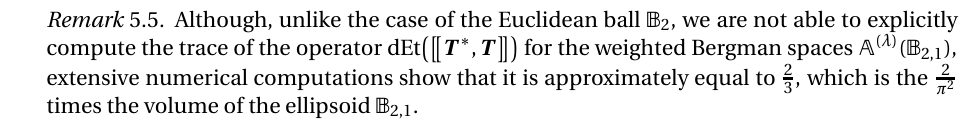
\includegraphics[width=0.96\textwidth]{figures/source_numerical_crop.png}
\caption{Source Remark~5.5 reports only numerical evidence for $2/3$
(PDF page 28).}
\end{figure}

\begin{figure}[H]
\centering

\includegraphics[width=0.96\textwidth]{figures/source_conjecture_crop.png}
\caption{The sharp spectral-volume bound in source Conjecture~5.6
(PDF page 29).}
\end{figure}

\section{The model and result}

For $\lambda>3$, the source defines the inner product by the measure
\[
 (1-|z_1|^2-|z_2|)^{\lambda-4}\,d\nu(z)
 \quad\text{on}\quad
 \mathbb B_{2,1}=\{(z_1,z_2)\in\C^2:|z_1|^2+|z_2|<1\}.
\]
The normalized monomials $\phi_{m,n}$, $m,n\ge0$, form an orthonormal basis.
Put $s=m+2n+\lambda$.  The source's norm formula gives
\[
 M_{z_1}\phi_{m,n}=\sqrt{\frac{m+1}{s}}\,\phi_{m+1,n},
 \qquad
 M_{z_2}\phi_{m,n}=
 \sqrt{\frac{(2n+2)(2n+3)}{s(s+1)}}\,\phi_{m,n+1}.
 \tag{3}
\]

\begin{theorem}[Exact ellipsoid trace]
\label{thm:main}
For every $\lambda\ge4$, let $M=(M_{z_1},M_{z_2})$ act on
$\mathbb A^{(\lambda)}(\mathbb B_{2,1})$.  Then
\[
 \tr\dEt\bigl([[M^*,M]]\bigr)=\frac23
 =\frac{2!}{\pi^2}\,\nu(\mathbb B_{2,1}).
\]
Consequently, source Conjecture~5.6 holds with equality for this entire
one-parameter family.
\end{theorem}

\section{Diagonalization}

Write $C_{ij}=[M_{z_j}^*,M_{z_i}]$ and $D=\dEt(C)$.  The two diagonal
commutators in (1) have respective eigenvalues
\[
 c_{11}=\frac{2n+\lambda-1}{s(s-1)},
 \qquad
 c_{22}=\frac{(2n+2)(2n+3)}{s(s+1)}
 -\frac{(2n)(2n+1)}{(s-2)(s-1)}.
 \tag{4}
\]
The mixed commutators move one step along the diagonals of the lattice.  The
squared coefficients contributing to $C_{12}C_{21}$ and $C_{21}C_{12}$ are
\[
 p^2=\frac{4(m+1)(2n)(2n+1)}{(s-1)s^2(s-2)^2},
 \qquad
 q^2=\frac{4m(2n+2)(2n+3)}{s(s+1)^2(s-1)^2}.
 \tag{5}
\]
Thus $D$ is diagonal and
\[
 D\phi_{m,n}=\chi_{m,n}\phi_{m,n},
 \qquad
 \chi_{m,n}=2c_{11}c_{22}-p^2-q^2.
 \tag{6}
\]
Expanding (6) agrees identically with the four-term formula for
$\chi_{\boldsymbol\alpha}$ printed on source page 28.  The source proves
$D\ge0$ for $\lambda\ge4$ \cite[Theorem preceding Remark~5.5]{MPS}, so all
$\chi_{m,n}$ are nonnegative.

\section{Exact telescoping}

Group the lattice by the weighted degree $m+2n$.  For $r\ge0$, set
\[
 B_r=\sum_{n=0}^{r}\chi_{2r-2n,n}
     +\sum_{n=0}^{r}\chi_{2r+1-2n,n}.
 \tag{7}
\]
We now give a rational certificate for the sum.  Put $x_r=\lambda+2r$ and
\[
\begin{aligned}
a&=-\frac{(\lambda-4)(\lambda-2)(\lambda^2-8\lambda+18)}{24},&
a_0&=-\frac{(\lambda-2)(2\lambda^2-11\lambda+18)}6,\\
b&=-\frac{(\lambda-3)(\lambda-1)(\lambda^2-6\lambda+11)}6,&
c&=\frac{3\lambda^4-30\lambda^3+96\lambda^2-88\lambda-28}{24},\\
c_0&=-\frac{3\lambda^4-30\lambda^3+96\lambda^2-96\lambda-8}{12},&
e&=\frac{2(2\lambda-5)}3.
\end{aligned}
\tag{8}
\]
Define
\[
 F_r=\frac a{(x_r-2)^2}+\frac{a+a_0}{x_r^2}
 +\frac b{(x_r-1)^2}+\frac c{x_r-2}
 +\frac{c+c_0}{x_r}+\frac e{x_r-1}.
 \tag{9}
\]

\begin{lemma}[Telescoping certificate]
For every $r\ge0$ and $\lambda\ge4$,
\[
 B_r=F_r-F_{r+1},\qquad F_0=\frac23,\qquad \lim_{r\to\infty}F_r=0.
\]
\end{lemma}

\begin{proof}
Substitute $m=2r-2n$ and $m=2r+1-2n$ into (4)--(6), sum the resulting
rational functions for $0\le n\le r$, and collect the partial fractions with
denominators $x_r+j$, $-2\le j\le2$.  The squared-denominator coefficients at
$x_r-2,x_r,x_r+2$ sum to zero, as do the first-order coefficients; the odd
terms occur in opposite pairs at $x_r-1,x_r+1$.  The result is exactly the
forward difference of (9).  Direct substitution and cancellation give
$F_0=2/3$.  Each paired first-order term in (9) cancels at infinity, and the
remaining expression is $O(r^{-1})$, so $F_r\to0$.

All three identities are exact rational identities.  The accompanying SymPy
script expands (6), checks it against the source formula, performs the two
finite sums in (7), and verifies
$B_r-(F_r-F_{r+1})=0$, $F_0-2/3=0$, and $\lim F_r=0$ symbolically.
\end{proof}

\begin{proof}[Proof of Theorem~\ref{thm:main}]
Because $D\ge0$, Tonelli's theorem permits the grouping (7).  The certificate
therefore yields
\[
 \tr D=\sum_{m,n\ge0}\chi_{m,n}
 =\sum_{r=0}^{\infty}(F_r-F_{r+1})=F_0=\frac23.
\]
Finally, polar coordinates give
\[
\begin{aligned}
\nu(\mathbb B_{2,1})
&=4\pi^2\int_0^1 r_1
   \int_0^{1-r_1^2}r_2\,dr_2\,dr_1
=\frac{\pi^2}{3}.
\end{aligned}
\]
Hence $(2!/\pi^2)\nu(\mathbb B_{2,1})=2/3$, as claimed.
\end{proof}

\section{Scope, verification, and novelty}

The theorem resolves the exact computation highlighted in source
Remark~5.5, but it does not prove (2) for every tuple in
$BS_{m,\vartheta}(\Omega)$.  Eight upgrade attempts examined affine
covariance, sums and tensor products, cyclic jet extensions, general
Helton--Howe formulas, proper monomial maps, and discrete Monge--Amp\`ere
interpretations.  The main obstruction is that the $BS$ hypotheses control
only the top-degree generalized commutator; they do not give the pairwise
Schatten estimates or a bounded-multiplicity principal function needed by
known trace-volume formulas.

\paragraph{Verification notes.}
Review should focus on (i) the weight calculation (3), (ii) the mixed-shift
coefficients (5), and (iii) the finite rational identity in the telescoping
lemma.  The symbolic script is a certificate, not a numerical experiment:
all checks occur over the rational-function field $\mathbb Q(\lambda,r)$.
The use of nonnegative eigenvalues and Tonelli follows from the source's
$\lambda\ge4$ positivity theorem.

\paragraph{Novelty check.}
On 11 August 2026, the four run indexes were searched for arXiv:2012.11115,
``determinant trace'', ``ellipsoid'', and ``$2/3$''.  Exact-title and
exact-formula web/arXiv searches found no proof or counterexample.  Most
significantly, Pramanick's revised 2025 thesis restates the bound as
Conjecture~3.19 and still describes the ellipsoid value as numerical evidence
\cite{Pramanick}.  Later weighted-Bergman Helton--Howe formulas found in the
search concern the unit ball, not this branched ellipsoid model
\cite{TWZ}.  Novelty confidence is moderate-high.

\paragraph{Human-review recommendation.}
Review as a substantial partial result.  It rigorously settles the source's
only non-ball test family and confirms the sharp constant, while making no
claim that the full $BS_{m,\vartheta}$ conjecture is solved.

\begin{thebibliography}{9}

\bibitem{MPS}
G.~Misra, P.~Pramanick, and K.~B.~Sinha,
\emph{A trace inequality for commuting tuple of operators},
arXiv:2012.11115, Theorem~5.4, Remark~5.5, and Conjecture~5.6.

\bibitem{Pramanick}
P.~Pramanick,
\emph{Trace Estimate for the Determinant Operator and Generalized
Commutator}, revised doctoral thesis, Indian Institute of Science, 2025,
Conjecture~3.19.

\bibitem{TWZ}
X.~Tang, Y.~Wang, and D.~Zheng,
\emph{Helton--Howe trace, Connes--Chern character and quantization},
arXiv:2204.04337.

\bibitem{HH}
J.~W.~Helton and R.~E.~Howe,
\emph{Traces of commutators of integral operators},
Acta Math. 135 (1975), 271--305.

\end{thebibliography}

\end{document}
